\section{ノイズの測定}
\subsection{解析方法}
図\ref{fg:Noise_analysis} は、横軸が時間で縦軸が波高のグラフに、LGADから得られる信号をプロットした2次元ヒストグラムである。
このヒストグラムから信号のない時間領域である50 ns から54 ns の範囲をx軸で射影したヒストグラムが 図\ref{fg:Noise_hist} である。
このヒストグラムの標準偏差をノイズとして、LGADとPINのノイズの電圧依存性を測定した。

\begin{figure}[h]
    \begin{minipage}[b]{0.5\linewidth}
        \centering
        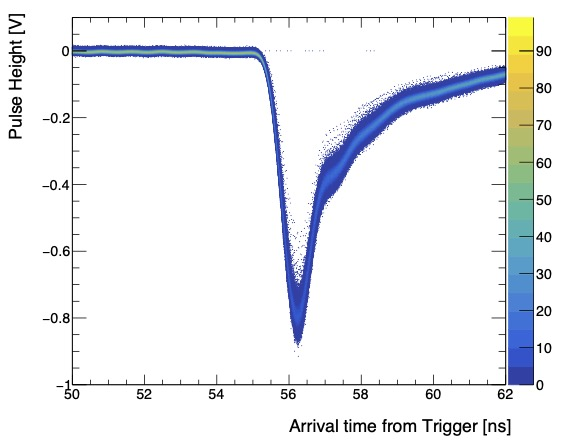
\includegraphics[width=8cm]{fig/ch5/noisevstime.jpg}
        \subcaption[波高と時間の2次元ヒストグラム]{波高と時間の2次元ヒストグラム\\横軸が時間、縦軸が波高}
        \label{fg:Noise_analysis}
    \end{minipage}
    \begin{minipage}[b]{0.5\linewidth}
        \centering
        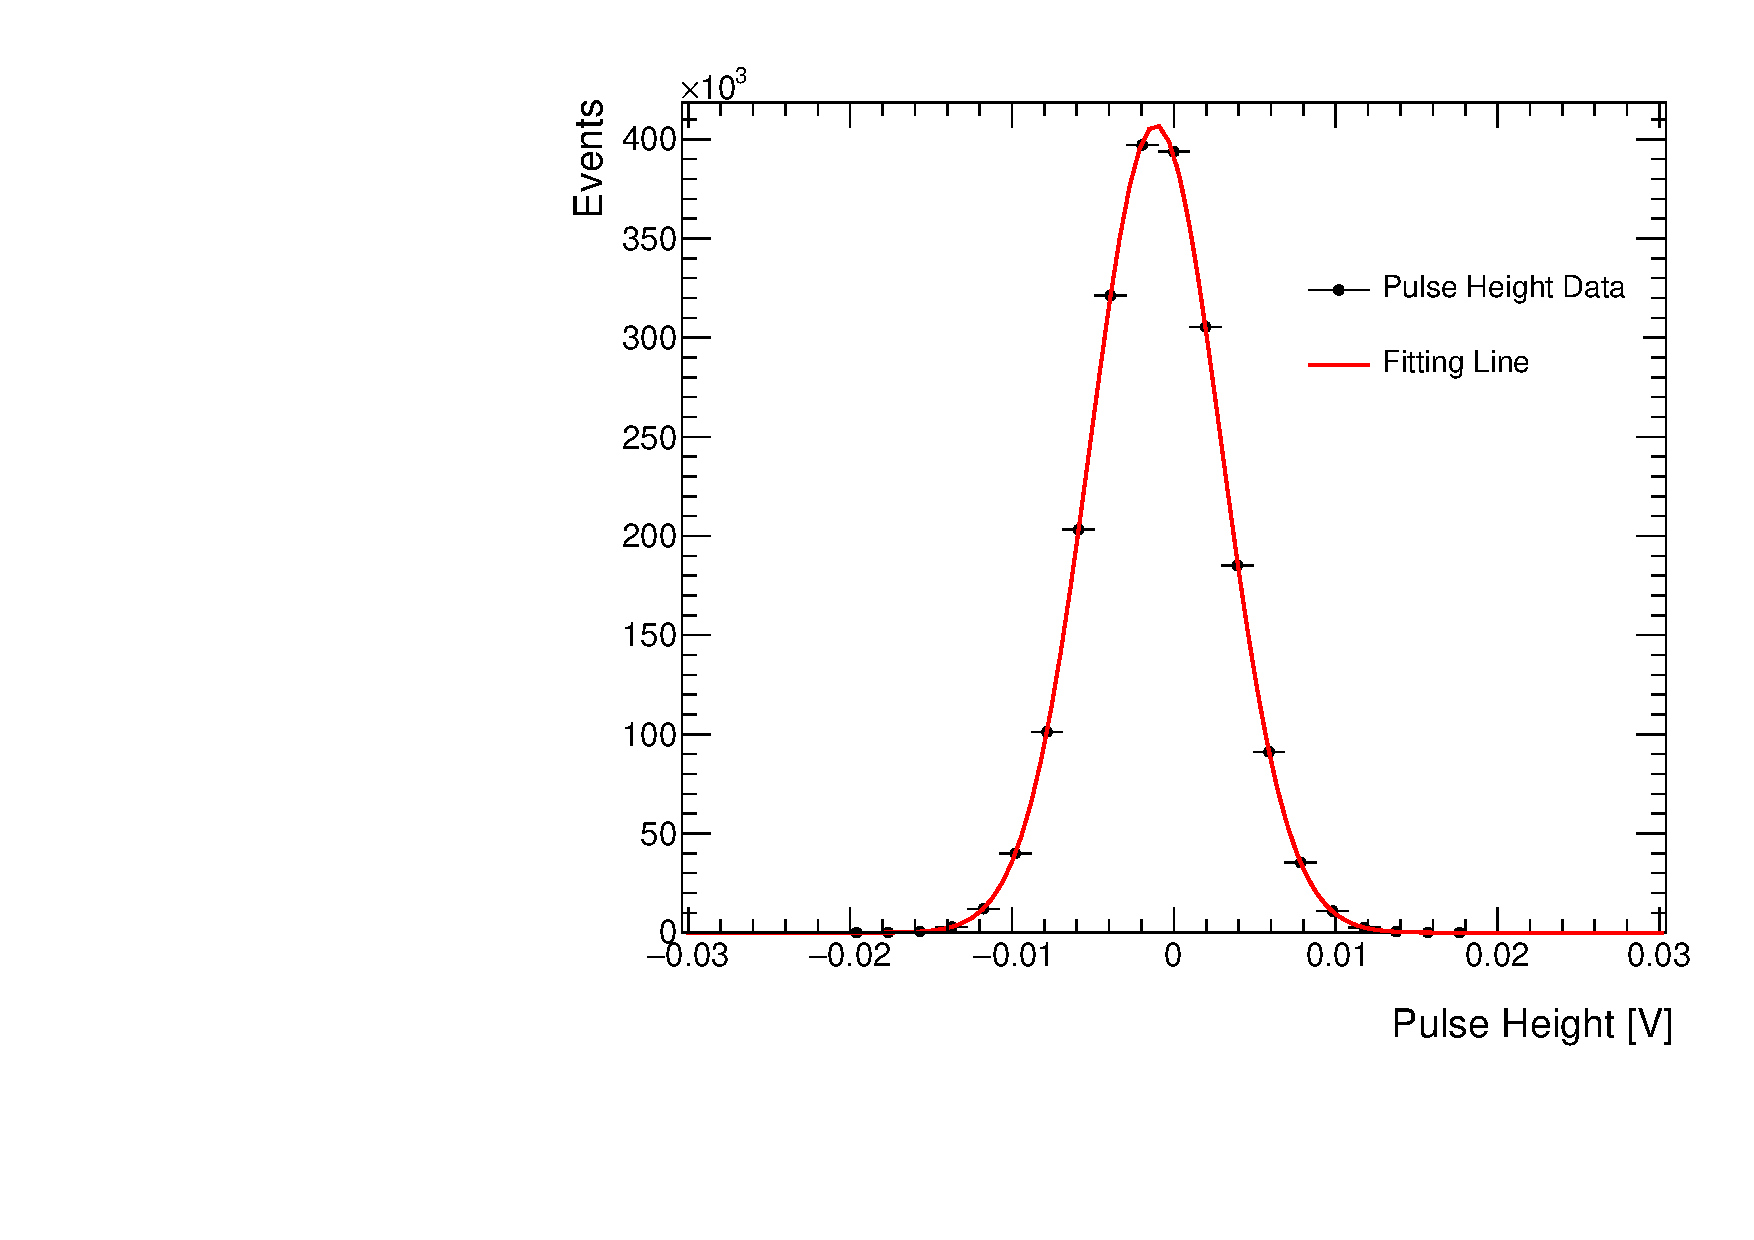
\includegraphics[width=8cm]{fig/graph/noise_hist.pdf}
        \subcaption[ノイズのヒストグラム]{ノイズのヒストグラム 横軸が波高}
        \label{fg:Noise_hist}
    \end{minipage}
    \caption[ノイズの解析方法]{ノイズの解析方法\\(a)のy軸を50 ns から54 nsの間で射影したのが(b)のヒストグラム\\(b)のヒストグラムの標準偏差をノイズとした。}
\end{figure}

\subsection{ノイズの測定結果}
LGADとPINのノイズの電圧依存性を 図\ref{fg:NoisevsBias} に示す。横軸が電圧で縦軸がノイズである。青点がPINで赤点がLGADの測定値を表している。
ノイズが一定になっている領域を見ると、PINのノイズは約2.6 mVに対して、LGADのノイズは約4 mVで、PINと比べて約1.6倍大きかった。
そのため、増幅層がない検出器と比べて、増幅層がある検出器はノイズが大きくなることがわかった。
また、200 VではLGADのノイズが急激に上昇し、およそ4.7 mVになることがわかった。
これは、図\ref{fg:IV_temp} の電流電圧特性を見ると、200 Vでは電子雪崩の影響が非常に大きくなることがわかる。
そのため、ノイズが大きくなる原因は、電子雪崩が生じることで暗電流が増加するためであると考える。


\begin{figure}[h]
    \centering
    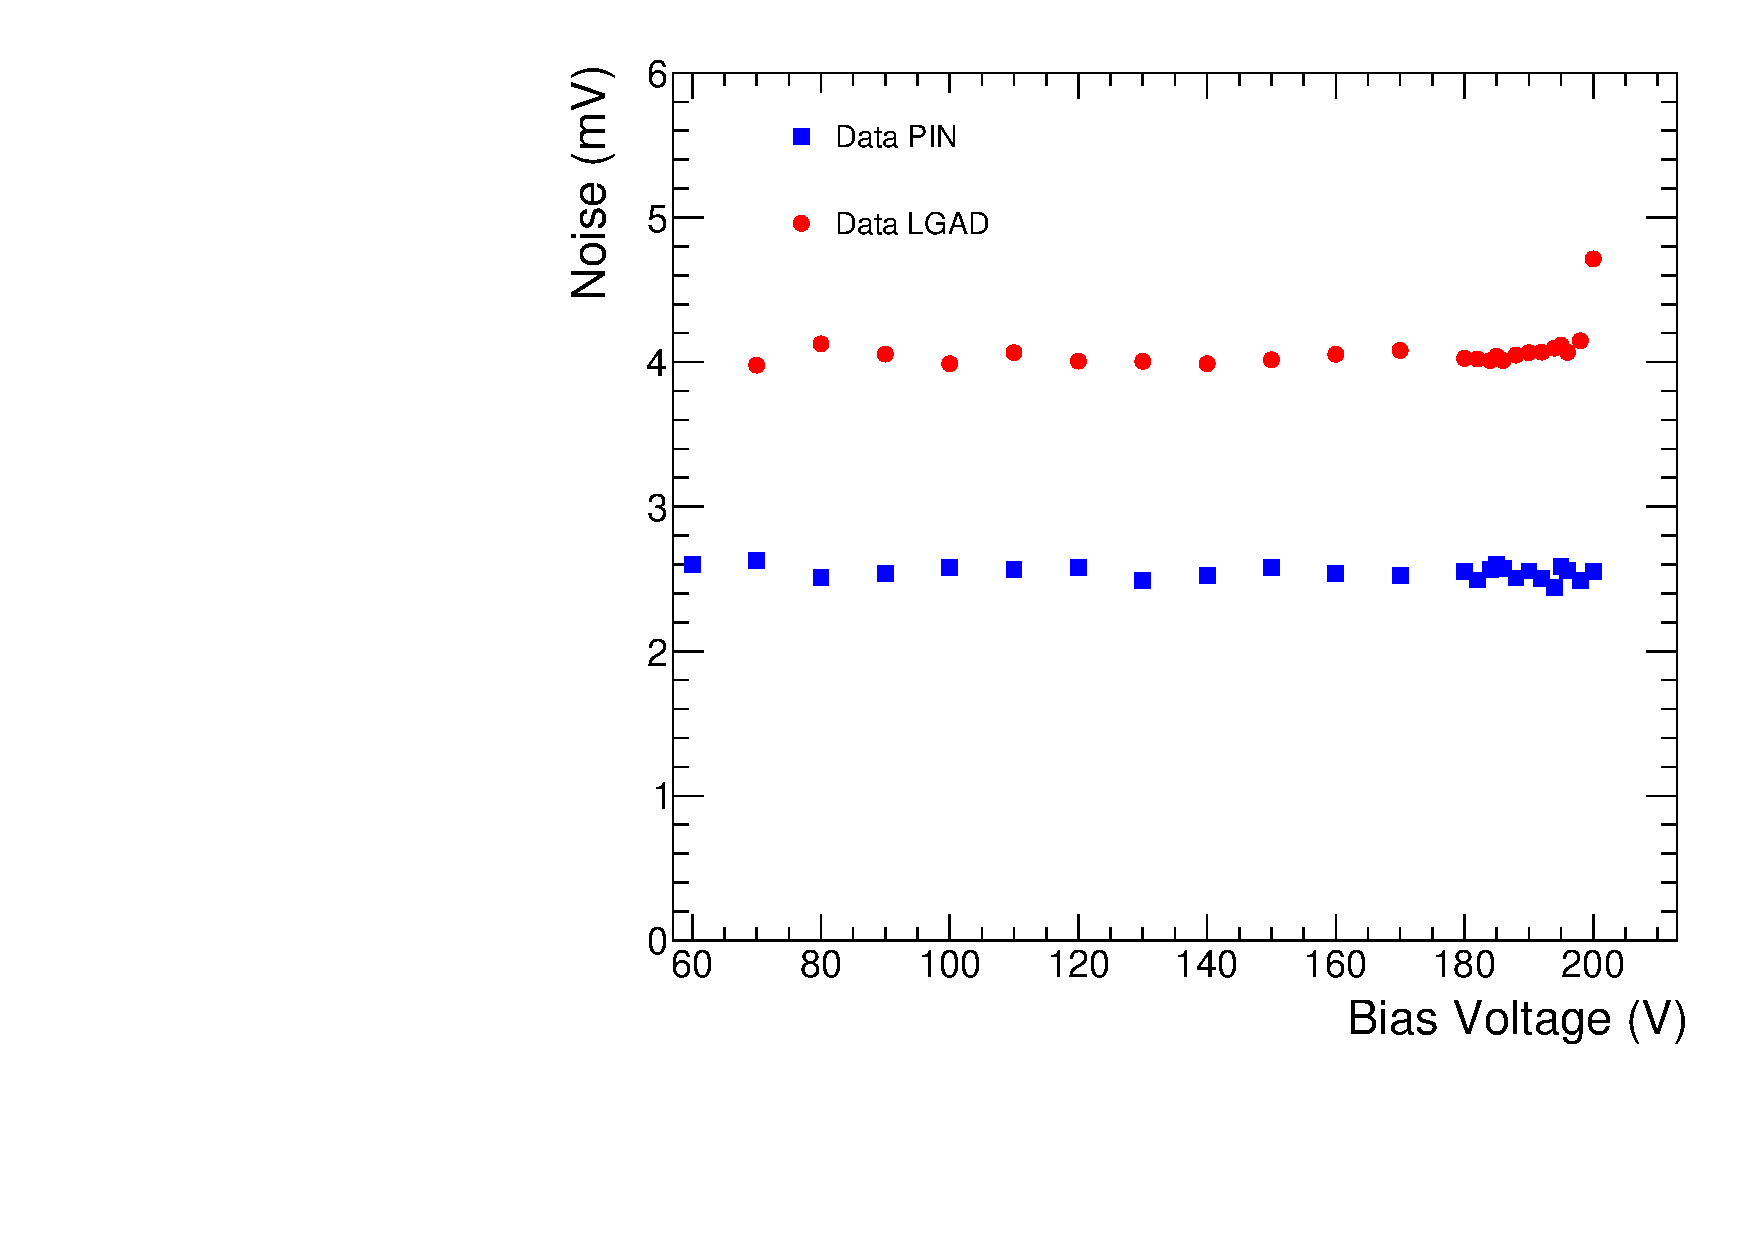
\includegraphics[width=8cm]{fig/graph/NoisevsVoltage.pdf}
    \caption[AC-LGAD検出器のノイズの電圧依存性]{AC-LGAD検出器のノイズの電圧依存性\\横軸が電圧で縦軸がノイズ、青点がPINで赤点がLGADの測定値}
    \label{fg:NoisevsBias}
\end{figure}

